\documentclass[11pt]{article}
\usepackage{setspace}  % To use linespacing
\usepackage{indentfirst} % Indents first line after sections
\usepackage{amssymb} % For \mathbb
\usepackage{enumerate} % For changing labels of enumerate
\usepackage[margin=1in]{geometry} % For editing margins
\usepackage{tikz} % Tikz drawing for graphs
\usetikzlibrary{arrows.meta} % Allows customizing arrows

\usepackage{amsmath}

% Make new commands
\newcommand{\N}{\mathbb{N}}
\newcommand{\R}{\mathbb{R}}
\newcommand{\Z}{\mathbb{Z}}
\newcommand{\abs}[1]{\left|#1\right|}
\newcommand{\fivespace}{\space\space\space\space\space}

% Start main document
\begin{document}
\onehalfspacing
\hfill Frank Cline

\hfill Math 307

\hfill HW 2

% Sections
% 3.1 # 4, 6, 7, 10
% 3.2 # 2, 3, 6, 8, 16
% 3.3 16 cd, 18 cd

% SECTION 3.1 # 4, 6, 7, 10
\section*{3.1}

\begin{enumerate}
\setcounter{enumi}{3}
\item The following relations are defined on $N$.
	\begin{enumerate}
	\item Write the relation $R_1$ defined by $(m,n)\in R_1$ if $m+n=5$ as a set of ordered pairs.\\
	$R_1=\{(0,5),(1,4),(2,3),(3,2),(4,1),(5,0)\}$
	\item Do the same for $R_2$ defined by max$\{m,n\}=2$.\\
	$R_2=\{(0,2),(1,2),(2,2),(2,1),(2,0)\}$
	\item The relations $R_3$ defined by min$\{m,n\}=2$ consists of infinitely many ordered pairs. List five 	of them.\\
	\{(2,3),(2,4),(2,5),(2,6),(2,7)\}
	\end{enumerate}
\setcounter{enumi}{5}
\item Consider the relation $R$ on $\Z$ defined by $(m,n)\in R$ if and only if $m^3-n^2\equiv 0$ mod$(5)$. Which of the properties $(R),(AR),(S),(AS)$, and $(T)$ are satisfied by $R$?
	\begin{itemize}
	\item $R$ does not satisfy $(R)$ because if $(m,n)=(3,3)$ then $3^3-3^2=27-9=18$ and $5\nmid18$, so 3 is not related to 			itself. Thus it's not reflexive.
	\item $R$ does not satisfy $(AR)$ because if $m,n=5$ then $5^3-5^2=125-25=100$ and $5\mid100$, so 5 is related to 
	itself. Thus it's not antireflexive.
	\item $R$ does not satisfy $(S)$ because if $m=1,n=4$ then $1^3-4^2=1-16=-15$ and $5\mid-15$, so 1 is related to 4.
	if $m=4,n=1$ then $4^3-1^2=64-1=63$ and $5\nmid63$, so 4 is not related to 1. Since 1 is related to 4 
	and 4 is not related to 1, it's not symmetric.
	\item $R$ does not satisfy $(AS)$ because if $m=5,n=0$ then $5^3-0^2=125$ and $5\mid125$, so 5 is related to 0.
	if $m=0,n=5$ then $0^3-5^2=-25$ and $5\mid-25$, so 0 is related to 5. Since 0 is related to 5 and 5 is 
	related to 0, but $5\not=0$ it's not antisymmetric.
	\item $R$ satisfies $(T)$. 
	\end{itemize}
\item Define the "divides" relation $R$ on $\N$ by $(m,n)\in R$ if $m\mid n$.
	\begin{enumerate}
	\item Which of the properties $(R),(AR),(S),(AS),(T)$ does $R$ satisfy?\\
		\begin{itemize}
		\item $R$ satisfies $(R)$.
		\item $R$ does not satisfy $(AR)$ because if $m,n=5$ then $5\mid5$ thus $(5,5)\in R$.
		\item $R$ does not satisfy $(S)$ because if $m=5,n=10$ then $5\mid10$, but if $m=10,n=5$ then $10\nmid5$ thus 
		$(5,10)\in R$, but $(10,5)\not\in R$.
		\item $R$ satisfies $(AS)$.
		\item $R$ satisfies $(T)$.
		\end{itemize}
	\item Describe the converse relation $R^\gets$.\\
	$R^\gets$ is the relation on $\N$ by $(m,n)\in R^\gets$ if $n\mid m$.
	\item Which of the properties $(R),(AR),(S),(AS),(T)$ does the converse satisfy?
		\begin{itemize}
		\item $R^\gets$ satisfies $(R)$.
		\item $R^\gets$ does not satisfy $(AR)$ because if $m,n=5$ then $5\mid5$ thus \\$(5,5)\in 
		R^\gets$.
		\item $R^\gets$ does not satisfy $(S)$ because if $m=10,n=5$ then $5\mid10$, 
		but if $m=5,n=10$ then $10\nmid5$ thus $(5,10)\in R^\gets$, but $(10,5)\not\in R^\gets$.
		\item $R^\gets$ satisfies $(AS)$.
		\item $R^\gets$ satisfies $(T)$.
		\end{itemize}
	\end{enumerate}
\setcounter{enumi}{9}
\item Give an example of the relation that is:
	\begin{enumerate}
	\item antisymmetric and transitive but not reflexive.\\
	The relation $R$ on $\Z$ by $(m,n)\in R$ if and only if $m<n$.
	\item symmetric but not reflexive or transitive.\\
	The relation $R$ on the set $\{0,1,2,3\}$ by $(m,n)\in R$ if and only if $max(m,n)=3$.
	\end{enumerate}
\end{enumerate}

% SECTION 3.2 # 2, 3, 6, 8, 16
\section*{3.2}
\begin{enumerate}
\setcounter{enumi}{1}
\item Draw a picture of the digraph G with vertex set $V(G)=\{w,x,y,z\}$, edge set $E(G)=\{a,b,c,d,e,f,g\}$, and 
$\gamma$ given by the following table:\\\\
	\begin{tabular}{c|c c c c c c c}
		$e$ & $a$ & $b$ & $c$ & $d$ & $e$& $f$& $g$\\
		\hline
		\\
		$\gamma(e)$ & $(x,w)$ & $(w,x)$ & $(x,x)$ & $(w,z)$ & $(w,y)$ & $(w,z)$ & $(z,y)$\\
	\end{tabular}
	
	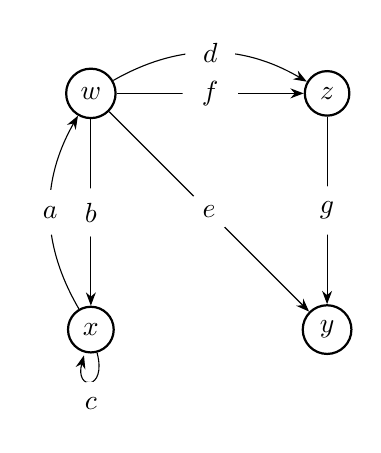
\begin{tikzpicture}
	\begin{scope}[every node/.style={circle,thick,draw}]
	    \node (x) at (0,-1) {$x$};
	    \node (w) at (0,2) {$w$};
	    \node (y) at (3,-1) {$y$};
	    \node (z) at (3,2) {$z$};
	\end{scope}

	\begin{scope}[>={Stealth[black]},
	              every node/.style={fill=white,circle},
	              every edge/.style={draw=black}]
	    	\path [->] (x) edge[bend left=30] node {$a$} (w); 
		\path [->] (w) edge node {$b$} (x);
	    	\path [->] (x) edge[loop below] node {$c$} (x);
		\path [->] (w) edge[bend left=30] node {$d$} (z);
	   	\path [->] (w) edge node {$e$} (y);
	    	\path [->] (w) edge node {$f$} (z);
	    	\path [->] (z) edge node {$g$} (y);
	\end{scope}
	\end{tikzpicture}
\item Which of the following vertex sequences describe paths in the digraph pictured in Figure$(7a)$?
	\begin{enumerate}
	\item $zyvwt$\\
	Yes
	\item $xzwt$\\
	Yes
	\item $vstx$\\
	No
	\item $zysu$\\
	No
	\item $xzyvs$\\
	Yes
	\item $suxt$\\
	No
	\end{enumerate}
\setcounter{enumi}{5}
\item There are four basic blood types: A, B, AB, and O. Type O can donate to any of the four types. A and B can donate to AB as 
well as their own types. AB can only donate to AB. Draw a digraph that presents this information. Is the digraph acyclic?\\
	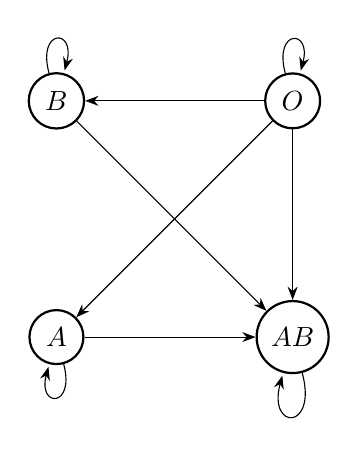
\begin{tikzpicture}
	\begin{scope}[every node/.style={circle,thick,draw}]
		\node (A) at (0,-1) {$A$};
	    	\node (B) at (0,2) {$B$};
	    	\node (AB) at (3,-1) {$AB$};
	    	\node (O) at (3,2) {$O$};
	\end{scope}
	
	\begin{scope}[>={Stealth[black]},
	              every node/.style={fill=white,circle},
	              every edge/.style={draw=black},
				every path/.style={->}]
		\path (O) edge (A);
		\path (O) edge (B);
		\path (O) edge (AB);
		\path (O) edge[loop above] (O);
		\path (A) edge (AB);
		\path (A) edge[loop below] (A);
		\path (B) edge (AB);
		\path (B) edge[loop above] (B);
		\path (AB) edge[loop below] (AB);
	\end{scope}
	\end{tikzpicture}

	\begin{itemize}
	\item Yes the digraph is acyclic because there are no cycles.
	\end{itemize}
\setcounter{enumi}{7}
\item Determine the reachability relation for the digraps in figures $6(a),(c)$, and $(d)$.
	\begin{itemize}
	\item If $R$ is the reachable relation on $V(G)$, then $R$ is the universal relation for figures $6(a),(c)$, and $(d)$.
	\end{itemize}
\setcounter{enumi}{15}
\item For the graph in Figure $8(a)$, give an example of each of the following. Be sure to specify the edge sequence 
and the vertex sequence.
	\begin{enumerate}
	\item a path of length 2 from $w$ to $z$.\\
	$w\xrightarrow{d} x\xrightarrow{f}z$
	\item a path of length 4 from $z$ to itself.\\
	$z\xrightarrow{e} x\xrightarrow{f} z\xrightarrow{g} x\xrightarrow{e}z$
	\item a path of length 5 from $z$ to itself.\\
	Impossible.
	\item a path of length 3 from $w$ to $x$.\\
	$w\xrightarrow{b} y\xrightarrow{b} w\xrightarrow{d} x$
	\end{enumerate}








\end{enumerate}


\end{document}